\chapter{Soft-Wall Model\label{sec:Soft-Wall-Model}}

The four-dimensional fields of QCD live in the five-dimensional
anti-de Sitter space, with a metric given by
\begin{equation}
ds^{2}g_{MN}dx^M dx^N=a^{2}(z)(\eta_{\mu\nu}dx^{\mu}dx^{\nu}+dz^{2}),
\end{equation}
where $a(z)=L/z$ is the warp factor and $L$ is the curvature radius of the anti-de Sitter space. 
The Minkowski metric is given by
\be
\eta_{\mu\nu}= \left( \begin{array}{cccc} 
 -1 & 0 & 0 & 0\\
  0 & 1 & 0 & 0\\
  0 & 0 & 1 & 0\\
  0 & 0 & 0 & 1
\end{array} \right).
\ee
The coordinate $z$ has a range $0\le z < \infty$.

The bulk coordinate $z$ is associated with inverse energy scales, with the ultraviolet limit of QCD represented by fields at $z\rightarrow0$\cite{kwee-lebed-pion}. 
The AdS/CFT dictionary \cite{maldacena,klebanov-witten} states that each operator $\mathcal{O}(x)$ in the 4D conformal field theory is associated with a bulk field $\psi(x,z)$. 
The values of the bulk fields at the UV boundary act as sources for the corresponding
4D currents. 
Global symmetries of the 4D field theory become gauged symmetries for the bulk fields. 

The field content of the 5D theory is dictated by the operators relevant to the chiral dynamics of QCD. 
The gauge fields $A_{L\,\mu},\, A_{R\,\mu}$ correspond to the left- and right-handed currents of the $SU(N_{f})_{L}\times SU(N_{f})_{R}$ chiral symmetry, where $N_{f}$ is the number of quark flavors in
the model. 
The scalar field $X$ is associated with the chiral operator $\bar{q}q$ \cite{stephanov-katz-son}. 
The masses of the bulk fields are set by the AdS/CFT relation \cite{colangelo-light-scalar-mesons} 
\be
m_{5}^{2}L^{2}=(\Delta-p)(\Delta+p-4), 
\ee
where $\Delta$ is the dimension of the $p$-form QCD operator. 
Table \ref{tab:Operators-and-fields} illustrates the fields and operators of our model, showing that the scalar field is the only field in this model that is not massless.

\begin{table}[htb]
\begin{center}
\begin{tabular}{|c|c|c|c|c|}
\hline 
4D Operator & 5D Field & $p$ & $\Delta$ & $m_{5}^{2}L^{2}$\\
\hline 
\hline 
$\bar{q_{L}}\gamma^{\mu}t^{a}q_{L}$ & $A_{L\,\mu}^{a}$ & 1 & 3 & 0\\
\hline 
$\bar{q_{R}}\gamma^{\mu}t^{a}q_{R}$ & $A_{R\,\mu}^{a}$ & 1 & 3 & 0\\
\hline 
$\bar{q}_{R}^{\alpha}q_{L}^{\beta}$ & $\frac{2}{z}X^{\alpha\beta}$ & 0 & 3 & -3\\
\hline 
\end{tabular}
\end{center}
\caption{Operators and fields of the model. The matrices $t^{a}$ are the generators of the $SU(N_{f})$ symmetry. 
\label{tab:Operators-and-fields}}
\end{table}

The simplest soft-wall action involving the fields from Table \ref{tab:Operators-and-fields}
is given in \cite{karch-katz-son-adsqcd} as 

\begin{equation}
S_{5}=\int d^{5}x\sqrt{-g}e^{-\Phi(z)}Tr\left[|DX|^{2}+m_{X}^{2}|X|^{2}+\frac{1}{4g_{5}^{2}}(F_{L}^{2}+F_{R}^{2})\right].
\end{equation}
The 5D gauge coupling constant $g_{5}$ is fixed by calculating the vector current two-point function using this model and then comparing this to the leading order result from QCD, leading to the identification $g_{5}^{2}=12\pi^{2}/N_{c}$ \cite{stephanov-katz-son}. 
The field $X$ includes both the scalar and pseudoscalar fields in a representation that will be discussed in Section \ref{sub:Pseudoscalar-Representation}.
The field strength tensors and covariant derivative are defined as
\ba
F_{L,R}^{MN}=\partial^{M}A_{L,R}^{N}-\partial^{N}A_{L,R}^{M}-i[A_{L,R}^{M},A_{L,R}^{N}]\\
D^{M}X=\partial^{M}X-iA_{L}^{M}X+iXA_{R}^{M}.
\ea
The physical vector ($V$) and axial-vector ($A$) fields, are defined in terms of the $L$ and $R$ gauge fields 
\ba
L^{M}&=&V^{M}+A^{M},\label{equLplusRV}\\
R^{M}&=&V^{M}-A^{M}.\label{equLminusRA}
\ea
Substituting equations (\ref{equLplusRV}) and (\ref{equLminusRA}) into the last field strength tensors,
\begin{eqnarray}
F_{L}^{2}+F_{R}^{2} &=& 2\left(\partial^{M}L^{N}\partial_{M}L_{N} - \partial^{M}L^{N}\partial_{N}L_{M}+\frac{1}{2}[L^{M},L^{N}][L_{M},L_{N}]\right)\nonumber\\
&+& 2\left(\partial^{M}R^{N}\partial_{M}R_{N} - \partial^{M}R^{N}\partial_{N}R_{M}+\frac{1}{2}[R^{M},R^{N}][R_{M},R_{N}]\right),\nonumber\\
&=& 4\left(\partial^{M}V^{N}\partial_{M}V_{N} - \partial^{M}V^{N}\partial_{N}V_{M}+\frac{1}{2}[V^{M},V^{N}][V_{M},V_{N}]\right)\nonumber\\
&+& 4\left(\partial^{M}A^{N}\partial_{M}V_{N} - \partial^{M}A^{N}\partial_{N}A_{M}+\frac{1}{2}[A^{M},A^{N}][A_{M},A_{N}]\right),\nonumber\\
&=& 2 \left(F_{V}^{2}+  F_{A}^{2}\right),\label{equchiraltovector}
\end{eqnarray}
where the vector and axial field-strength tensors have the form
\begin{eqnarray}
F_{V}^{MN}&=&\partial^{M}{V^{N}}-\partial^{N}{V^{M}}-\frac{i}{\sqrt{2}}[V^{M},V^{N}],\\
F_{A}^{MN}&=&\partial^{M}{A^{N}}-\partial^{N}{A^{M}}-\frac{i}{\sqrt{2}}[A^{M},A^{N}].
\end{eqnarray}
The covariant derivative can also be written in terms of the  vector and axial fields
\begin{equation}
D_{M}X=\partial_{M}X-i\{A_{M}^{a},X\}+i[V_{M}^{a},X].
\label{eq:covariant_der}
\end{equation}


The scalar field $X$ takes on a $z$-dependent vacuum expectation value (VEV), breaking the chiral symmetry. 
In a flavor-symmetric model, the VEV has the form 
\be
\langle X\rangle=\frac{\chi(z)}{2}I,
\ee
 where $I$ is the $N_{f}\times N_{f}$ identity matrix. 
From the AdS/CFT dictionary established in \cite{maldacena,klebanov-witten}, $\chi(z)$
has the ultraviolet asymptotic form
\begin{equation}
\lim_{z\rightarrow0}\chi(z)=m_{q}z+\sigma z^{3},\label{eq:VEV}
\end{equation}
where $m_{q}$ is the quark mass and $\sigma=\langle\bar{q}q\rangle$ is the chiral condensate, the variation of the vacuum energy with respect to $m_{q}$. 
In \cite{karch-katz-son-adsqcd}, it is shown that, when $\chi(z)$ is defined by (\ref{eq:VEV}) over the whole range of $z$, the chiral condensate is proportional to the quark mass.
Thus, the spontaneous and explicit chiral symmetry breaking terms are related, contrary to expectations.

As an example calculation, we can derive the mass spectrum of the vector $\rho$ mesons by varying the vector field and using the axial gauge condition $V_{z}=0.$ 
Varying the action, we find that 
\begin{eqnarray}
\delta \mathcal{S}_{V} &=& -\delta\left({\rm e}^{-\Phi}\sqrt{-g}g^{\mu\rho}g^{\nu\sigma}\left(\partial_{\mu}V_{\nu}\partial_{\rho}V_{\sigma} - \partial_{\mu}V_{\nu}\partial_{\sigma}V_{\rho}\right)+{\rm e}^{-\Phi}\sqrt{-g}g^{zz}g^{\mu\nu}\partial_{z}V_{\mu}\partial_{z}V_{\nu}\right) \nonumber\\
&=& -{\rm e}^{-\Phi}\sqrt{-g}g^{\mu\rho}g^{\nu\sigma}\left(\partial_{\mu}V_{\nu}\delta\partial_{\rho}V_{\sigma} - \partial_{\mu}V_{\nu}\delta\partial_{\sigma}V_{\rho}\right) - {\rm e}^{-\Phi}\sqrt{-g}g^{zz}g^{\mu\nu}\partial_{z}V_{\mu}\delta\partial_{z}V_{\nu}\nonumber\\
&=& {\rm e}^{-\Phi}a(z) (\partial^{2}V_{\mu}\delta V^{\mu} - \partial_{\mu}\partial^{\nu}V_{\nu}\delta V^{\mu}) + \partial_{z}\left({\rm e}^{-\Phi} a(z)\partial_{z} V_{\mu}\right)\delta V^{\mu}\nonumber\\
&=& \left({\rm e}^{-\Phi} a(z) \partial_{\nu}\partial^{\nu}V_{\mu} + \partial_{z}\left({\rm e}^{-\Phi} a(z)\partial_{z} V_{\mu}\right)\right)\delta V^{\mu},\label{equVectorstep}
\end{eqnarray}
 
We can separate out the $z-$dependence of the field: 
\be 
V_{\mu}^{n}=\mathcal{V}_{\mu}^{n}(x)V_{n}(z), 
\ee
where $V_{n}(z)$ are the Kaluza-Klein modes. 
The equation of motion is now one dimensional
\begin{equation}
-\partial_{z}^{2}V_{n}+\omega'\partial_{z}V_{n}=m_{V_{n}}^{2}V_{n},
\label{eq:vectorEOM1}
\end{equation}
where $\omega=\Phi(z)+\log z$, and ($'$) represents differentiation with respect to $z$. 
We can eliminate the first derivative of the field, bringing the equation of motion into Schrodinger-like form, using the substitution $V_{n}(z)=e^{\omega/2}v_{n}(z)$.
The equation of motion is now
\begin{equation}
-v_{n}^{''}+\left(\frac{1}{4}\omega^{'2}-\frac{1}{2}\omega^{''}\right)v_{n}=m_{V_{n}}^{2}v_{n}.\label{eq:EOM-vector-simple}
\end{equation}
This is the general method for finding the equations of motion for the various fields. 
Using the asymptotic form of the dilaton $\Phi=\lambda z^{2},$ the mass eigenvalues can be found exactly for this model. The equation of motion is now
\begin{equation}
-v_{n}^{''}+\left(\lambda z^{2}+\frac{3}{4z^{2}}\right)v_{n}=m_{n}^{2}v_{n}.
\end{equation}
The eigenvalues for this equation are $m_{n}^{2}=\lambda(4n+4)$ for $n=0,1,2,3,\dots$ 
The parameter $\lambda$ is set by matching this trajectory to experimental data. 

The equation of motion for the axial sector is derived using the same method, yielding
\begin{equation}
-a_{n}^{''}+\left(\frac{1}{4}\omega^{'2}-\frac{1}{2}\omega^{''}+g_{5}^{2}\frac{L^{2}}{z^{2}}\chi^{2}(z)\right)a_{n}=m_{V_{n}}^{2}a_{n}.\label{eq:EOM-axial-simple}
\end{equation}
The only difference from (\ref{eq:EOM-vector-simple}) is the presence of the $z$-dependent mass term involving the VEV. 
The significant drawbacks for this simple soft-wall model are the relatively poor modeling of the ground state and lower resonances and the lack of independent spontaneous and explicit chiral symmetry
breaking terms.


\section{Modified Soft-Wall Model\label{sub:Modified-Soft-Wall-Model}}

An improvement on the soft-wall model, suggested in \cite{karch-katz-son-adsqcd}, is adding higher-order terms of $X$ to the scalar potential, separating the spontaneous and explicit chiral symmetry breaking. 
The model established in \cite{gherghetta-kelley} adds a quartic scalar term to the action:
\begin{equation}
S_{5}=\int d^{5}x\sqrt{-g}e^{-\Phi(z)}Tr\left[|DX|^{2}+m_{X}^{2}|X|^{2}-\kappa|X|^{4}+\frac{1}{2g_{5}^{2}}(F_{A}^{2}+F_{V}^{2})\right],\label{equAction1}
\end{equation}
where $\kappa$ is a parameter to be fit to the data.
 Taking $X=X_{0}$ and varying (\ref{equAction1}), we find that $\chi(z)$ has the following nonlinear equation of motion:
\begin{equation}
\partial_{z}(a^{3}e^{-\Phi}\partial_{z}\chi(z))-a^{5}e^{-\Phi}\left(m_{X}^{2}\chi(z)-\frac{\kappa}{2}\chi^{3}(z)\right)=0.\label{eq:dilatonEOM}
\end{equation}
The VEV retains the same UV asymptotic form (\ref{eq:VEV}), while the non-restoration of chiral symmetry dictates that $\chi(z)\sim z$ in the infrared region. 
The VEV is parameterized so that it matches the expected asymptotic behavior. 
A suitable form was found and justified in \cite{gherghetta-kelley}
\begin{equation}
\chi(z)=\alpha z+\beta \mathrm{tanh}(\gamma z^{2})\label{eq:VEV-parametrization}
\end{equation}
with the parameters defined as follows
\[
\alpha=\frac{\sqrt{3}m_{q}}{g_{5}L},\qquad\beta=\sqrt{\frac{4\lambda}{\kappa L^{2}}}-\alpha,\qquad\gamma=\frac{g_{5}\sigma}{\sqrt{3}\beta}.
\]
 The quark mass and chiral condensate can each be taken to zero independently, and the non-restoration of chiral symmetry does not depend on eitherof these parameters. 
 Thus, the spontaneous and chiral symmetry breaking occur separately, as desired. 
Using (\ref{eq:VEV-parametrization}) in (\ref{eq:dilatonEOM}) we can solve for the dilaton field.

Equations of motion are then derived using the method of Section \ref{sec:Soft-Wall-Model}, and the equations of motion for the vector and axial fields have thesame form as \ref{eq:EOM-vector-simple} and (\ref{eq:EOM-axial-simple}), respectively. 
Due to the more complicated forms for $v$ and $\Phi$, the eigenvalues are not analytically solvable, so a numerical shooting method is used to calculate the mass spectra for the scalar, vector,
and axial sectors. 
The results for the vector mesons are shown in Figure \ref{fig:Vector}, and the scalar and axial sectors show similarly good results \cite{gherghetta-kelley}. 
These results reproduce the linear trajectories found in the simple soft-wall model \cite{karch-katz-son-adsqcd} for large $n$, while improving the agreement of the lower excitations with data.

\section{Pions in Soft-Wall AdS/QCD \label{sec:Pions}}

The mass spectrum for the pseudoscalar mesons was not found in the original paper \cite{gherghetta-kelley} because the equations of motion are coupled, second order differential equations, and because
of some subtleties that arise when considering the representation of the pseudoscalar field. 
The paper \cite{sui-pion} attempted to circumvent these problems by reducing the equations of motion to a single second-order equation, solvable by the shooting method, but their results seemed to miss
certain essential features of the pion spectrum. 
The authors later address this apparent discrepancy in \cite{sui-3flavor}.
This modified soft-wall model was later completed in the paper \cite{bartz-pions}, which clarified the discrepancies between two common representations of the pseudoscalar field, calculated the pion mass spectrum to good accuracy, and derived the Gell-Mann--Oakes--Renner relation from the model.

\subsection{Pseudoscalar Representation\label{sub:Pseudoscalar-Representation}}

As mentioned above, the field $X$ contains both the field representing the scalar mesons, $S,$ and the field representing the pseudoscalars, $\pi,$ as well as the VEV. 
There are two common ways to represent this field:
\ba
X_{e} &=& \left(\frac{\chi(z)}{2}+S(x,z)\right)Ie^{2i\pi_{e}(x,z)^{a}t^{a}}\\ \label{equXe}
X_{l} &=& \left(\frac{\chi(z)}{2}+S(x,z)\right)I+i\pi_{l}(x,z)^{a}t^{a}\label{equXl}
\ea
with $I$ the $N_{f}\times N_{f}$ identity matrix and $t^{a}$ the $SU(N_{f})$ generators. 
We will refer to $X_{e}$ as the exponential representation and $X_{l}$ as the linear representation. 
Apparent differences between the representations arise as we note that $\pi_{e}$
and $\pi_{l}$ have different dimensionality. 
In addition, the linear representation has a quartic interaction term in the Lagrangian, in contrast to the exponential representation. 
Equations of motion derived from each representation are shown to be equivalent.

\subsubsection{Exponential Representation}

Let us take (\ref{equXe}) and substitute it into (\ref{equAction1}), keeping terms that include the field $\pi(\mathbf{x},z)$, as well as terms that will mix with $\pi$, 
\ba
\mathcal{L}_{e} & = & -\sqrt{-g}{\rm e}^{-\Phi(z)}\frac{1}{2}\delta^{ab}\Big(g^{MN}(\chi^{2}\,\partial_{M}\pi\partial_{N}\pi+\chi^{2}A_{M}A_{N}-2\chi^{2}\partial_{M}\pi A_{N})\nonumber \\
 &  & +\frac{g^{MP}g^{NR}}{g_{5}^{2}}(\partial_{M}A_{N}\partial_{P}A_{R}-\partial_{M}A_{N}\partial_{R}A_{P})\Big)+\dots\label{start}
\ea
We work in the axial gauge, $A_{z}=0$, and separate $A_{\mu}$ into its transverse and longitudinal components: $A_{\mu}=A_{\mu\perp}+\partial_{\mu}\varphi,$ where $\partial_{\mu}A_{\perp}^{\mu}=0$. 
Separating (\ref{start}) explicitly into regular 4D components and extra-dimensional terms,
and expressing it in terms of the longitudinal part of $A_{\mu}$ gives 
\ba
\mathcal{L}_{e} & = & -\frac{1}{2}{\rm e}^{-\Phi(z)}\Big[\sqrt{-g}g^{\mu\nu}(\chi^{2}\partial_{\mu}\pi\partial_{\nu}\pi+\chi^{2}\partial_{\mu}\varphi\partial_{\nu}\varphi-2\chi^{2}\partial_{\mu}\pi\partial_{\nu}\varphi)\nonumber \\
 &  & +\sqrt{-g}g^{zz}\chi^{2}\partial_{z}\pi\partial_{z}\pi\ +\frac{\sqrt{-g}g^{zz}g^{\mu\nu}}{g_{5}^{2}}(\partial_{z}\partial_{\mu}\varphi\partial_{z}\partial_{\nu}\varphi)\Big].\label{equLproper}
\ea
Varying (\ref{equLproper}) with respect to $\pi$ and  performing a Kaluza-Klein decomposition, as above in (\ref{eq:vectorEOM1}), expressing the system of equations in terms of its $z$-dependent parts. 
\begin{equation}
e^{\Phi}\partial_{z}\left(\frac{e^{-\Phi}\chi^{2}}{z^{3}}\partial_{z}\pi_{n}\right)+\frac{\chi^{2}m_{n}^{2}}{z^{3}}(\pi_{n}-\varphi_{n})=0.\label{equOne}
\end{equation}
Varying (\ref{equLproper}) with respect to $\varphi$ and breaking it down into KK modes gives the second equation of motion 
\begin{equation}
{\rm e}^{\Phi}\partial_{z}\left(\frac{{\rm e}^{-\Phi}}{z}\partial_{z}\varphi{}_{n}\right)+\frac{g_{5}^{2}L^{2}\chi^{2}}{z^{3}}(\pi_{n}-\varphi_{n})=0.\label{equTwo}
\end{equation}
As usual, we express (\ref{equOne}) and (\ref{equTwo}) in a Schrodinger-like form,
\ba
\pi & = & {\rm e}^{f(z)}\tilde{\pi}\quad\quad\quad f(z)=\Phi(z)+\log{\frac{z^{3}}{\chi(z)^{2}}}\\
\varphi & = & {\rm e}^{g(z)}\tilde{\varphi}\quad\quad\quad g(z)=\Phi(z)+\log{z}.
\ea
After reverting back to the notation $\tilde{\pi}\rightarrow\pi$ and $\tilde{\varphi}\rightarrow\varphi$ the equations of motion become
\begin{eqnarray}
 &  & -\pi_{n}''+\left(\frac{\Phi'^{2}}{4}-\frac{\Phi''}{2}-\frac{\Phi'\chi'}{\chi}+\frac{3\Phi'}{2z}+\frac{15}{4z^{2}}-\frac{3\chi'}{\chi z}+\frac{\chi''}{\chi}-m_{n}^{2}\right)\pi_{n}=-m_{n}^{2}\frac{\chi^{2}L^{2}}{z^{2}}\varphi_{n}\label{equSchexppi}\\
 &  & -\varphi_{n}''+\left(\frac{\Phi'^{2}}{4}-\frac{\Phi''}{2}+\frac{\Phi'}{2z}+\frac{3}{4z^{2}}+\frac{g_{5}^{2}\chi^{2}L^{2}}{z^{2}}\right)\varphi_{n}=g_{5}^{2}\pi_{n}\label{equSchexpphi}
\end{eqnarray}



\subsubsection{Linear Representation}

When considering the linear representation of the pseudoscalar field (\ref{equXl}), there are terms quadratic and quartic in $\pi$ that were not present in the exponential representation. 
After making the appropriate substitutions in the Lagrangian, it becomes 
\begin{eqnarray}
\mathcal{L}_{l} & = & -\frac{1}{2}{\rm e}^{-\Phi}\sqrt{-g}\Big(g^{\mu\nu}\partial_{\mu}\pi\partial_{\nu}\pi+g^{zz}\partial_{z}\pi\partial_{z}\pi-2vg^{\mu\nu}\partial_{\mu}\pi\partial_{\nu}\varphi+m_{X}^{2}\pi^{2}-\frac{\kappa}{2}\chi^{2}\pi^{2}\nonumber \\
 & + & g^{\mu\nu}\chi^{2}\partial_{\mu}\varphi\partial_{\nu}\varphi+\frac{g^{\mu\nu}g^{zz}}{g_{5}^{2}}\partial_{z}\partial_{\mu}\varphi\partial_{z}\partial_{\nu}\varphi\Big).
\end{eqnarray}
Following the same procedure as above, we derive two coupled equations.
Varying with respect to $\varphi$ produces 
\begin{equation}
{\rm e}^{\Phi}\partial_{z}\left(\frac{{\rm e}^{-\Phi}}{z}\partial_{z}\varphi_{n}\right)+\frac{g_{5}^{2}L^{2}\chi}{z^{3}}\left(\pi_{n}-\chi\varphi_{n}\right)=0.\label{equphi}
\end{equation}
Varying with respect to $\pi$ gives the second equation of the linear representation 
\begin{equation}
z^{3}{\rm e}^{\Phi}\partial_{z}\left(\frac{{\rm e}^{-\Phi}}{z^{3}}\partial_{z}\pi_{n}\right)-\left(\frac{m_{X}^{2}}{z^{2}}-\frac{\kappa L^{2}\chi^{2}}{2z^{2}}\right)\pi_{n}+m_{n}^{2}\pi_{n}=m_{n}^{2}\chi\varphi_{n}.\label{equpi}
\end{equation}
 We can express (\ref{equphi}) and (\ref{equpi}) in a Schrodinger-like form as above %
with the substitutions 
\begin{eqnarray}
\pi_{n} & = & {\rm e}^{f}\tilde{\pi_{n}}\quad\quad\quad f=\frac{\Phi}{2}+\frac{3}{2}\log{\frac{z}{L}}\\
\varphi_{n} & = & {\rm e}^{g}\tilde{\varphi_{n}}\quad\quad\quad g=\frac{\Phi}{2}+\frac{1}{2}\log{\frac{z}{L}}.
\end{eqnarray}
Simplifying the equations and reverting back to the notation $\tilde{\pi_{n}}\rightarrow\pi_{n}$ and $\tilde{\varphi_{n}}\rightarrow\varphi_{n}$ for simplicity, we find  
\begin{eqnarray}
 &  & -\varphi_{n}''+\left(\frac{\Phi'^{2}}{4}-\frac{\Phi''}{2}+\frac{3}{4z^{2}}+\frac{\Phi'}{2z}+\frac{g_{5}^{2}L^{2}\chi^{2}}{z^{2}}\right)\varphi_{n}=\frac{g_{5}^{2}L\chi}{z}\pi_{n}\label{equSchphi}\\
 &  & -\pi_{n}''+\left(\frac{\Phi'^{2}}{4}-\frac{\Phi''}{2}+\frac{3}{4z^{2}}+\frac{3\Phi'}{2z}-\frac{\kappa L^{2}\chi^{2}}{2z^{2}}-m_{n}^{2}\right)\pi_{n}=-m_{n}^{2}\frac{\chi L}{z}\varphi_{n}\label{equSchpi}
\end{eqnarray}

\subsection{Representation Equivalence}

The pseudoscalar field representation should not affect the physical results obtained from the model. 
It is therefore desirable to show that the equations of motion derived from the two representations are equivalent.

We begin by expanding $X_{e}$ to first order in the fields 
\begin{eqnarray}
X_{e} & = & \left(\frac{\chi}{2}+S\right)(1+2i\pi_{e}+\ldots)\nonumber \\
 & = & \frac{\chi}{2}+S+i\pi_{e}\chi.\label{equXexpand}
\end{eqnarray}
Comparing (\ref{equXexpand}) to (\ref{equXl}), we surmise that $\pi_{e}\chi(z)\rightarrow\pi_{l}$ is the relationship between the two representations. 
Let us substitute
$\pi_{e}\rightarrow\pi_{l}/\chi(z)$ into the equations of motion of the exponential representation and attempt to obtain the equations of motion of the linear representation. 
The substitution into (\ref{equTwo}) immediately yields 
\begin{equation}
{\rm e}^{\Phi}\partial_{z}\left(\frac{{\rm e}^{-\Phi}}{z}\partial_{z}\varphi\right)+\frac{g_{5}^{2}\chi}{z^{3}}(\pi_{l}-\chi\varphi)=0,
\end{equation}
which is equivalent to (\ref{equphi}) as expected. 
Showing the equivalence of the other two equations requires a bit more work. 
First we substitute for $\pi_{e}$ in (\ref{equOne}) and then simplify the expression,
\begin{equation}
\frac{z^{3}{\rm e}^{\Phi}}{\chi}\partial_{z}\left(\frac{{\rm e}^{-\Phi}\chi^{2}}{z^{3}}\left(\frac{\pi_{l}'}{\chi}-\frac{\pi_{l}\chi}{\chi^{2}}\right)\right)+m_{n}^{2}(\pi_{l}-\chi\varphi)=0
\end{equation}
which becomes
\begin{equation}
\pi_{l}''-\left(\Phi'+\frac{3}{z}\right)\pi_{l}'-\frac{\pi_{l}}{\chi}\left(\chi''-\Phi'\chi'-\frac{3}{z}\chi'\right)+m_{n}^{2}(\pi_{l}-\chi\varphi)=0.\label{equOnemid}
\end{equation}
Recalling the equation of motion for $\chi(z)$ (\ref{eq:dilatonEOM}), which does not depend on the pseuodscalar representation: 
\begin{equation}
\chi''-\left(\Phi'+\frac{3}{z}\right)\chi'+\left(\frac{3}{z^{2}}+\frac{\kappa L^{2}\chi^{2}}{2z^{2}}\right)v=0.\label{equchi}
\end{equation}
Using (\ref{equchi}) in (\ref{equOnemid}), we find 
\begin{equation}
\pi_{l}''-\left(\frac{3}{z}+\Phi'\right)\pi_{l}'+\left(\frac{3}{z^{2}}+\frac{\kappa L^{2}\chi^{2}}{2z^{2}}\right)\pi_{l}+m_{n}^{2}\left(\pi_{l}-\chi\varphi\right)=0,
\end{equation}
which is equivalent to the other equation of motion of the linear representation (\ref{equpi}). 
The equations of motion are equivalent, confirming that physical results do not depend on the representation.

\subsection{Gell-Mann--Oakes--Renner Relation}

In this section we explore the Gell-Mann--Oakes--Renner relation numerically.
Inserting the established equivalence between the exponential and linear representations, $\pi_{e}=\pi_{l}/\chi(z)$, into (\ref{equOnemid}), we obtain 
\begin{equation}
\frac{g_{5}^{2}L^{2}\chi^{2}}{z^{2}}\partial_{z}\left(\frac{\pi_{l}}{\chi}\right)=m_{\pi}^{2}\partial_{z}\varphi\,.\label{eq:EOM-Modified}
\end{equation}
 Following the method of \cite{stephanov-katz-son}, we construct a perturbative solution in $m_{\pi}$ where $\varphi(z)=A(0,z)-1$ and use the established relation
\begin{equation}
f_{\pi}^{2}=-\left.L\frac{\partial_{z}A(0,z)}{g_{5}^{2}z}\right|_{z\rightarrow0.}\label{eq:fpi}
\end{equation}
Integrating (\ref{eq:EOM-Modified}) yields 
\begin{equation}
\frac{\pi(z)}{\chi(z)}=m_{\pi}^{2}\int_{0}^{z}du\,\frac{u^{3}}{\chi^{2}(u)}\frac{\partial_{z}A(0,u)}{g_{5}^{2}u}\,.
\end{equation}
The function $u^{3}/\chi^{2}(u)$ has significant support only at small values of $u\sim\sqrt{m_{q}/\sigma}$, where we may use (\ref{eq:fpi}) to relate the derivative on $A(0,u)$ to the pion decay constant, so that 
\begin{equation}
\frac{\pi_{l}}{\chi}=-\frac{m_{\pi}^{2}f_{\pi}^{2}}{2m_{q}\sigma}\,.\label{equPreGOR}
\end{equation}
We find that letting $\pi_{l}=-\chi(z)$ solves the axial-vector field's equation of motion 
\begin{equation}
{\rm e}^{\Phi}\partial_{z}\left(\frac{{\rm e}^{-\Phi}}{z}\partial_{z}A_{\mu}(q,z)\right)-\frac{q^{2}}{z}A_{\mu}(q,z)-\frac{g_{5}^{2}L^{2}\chi^{2}}{z^{3}}A_{\mu}(q,z)=0
\end{equation}
 in the region of small $z$ and as $q\rightarrow0$. 
 As a result, (\ref{equPreGOR}) becomes the expected Gell-Mann--Oakes--Renner (GOR)
relation, 
\begin{equation}
2m_{q}\sigma=m_{\pi}^{2}f_{\pi}^{2}\,.\label{eq:GOR}
\end{equation}

We solve for the ground-state pseudoscalar mass, $m_{\pi}$, for
differing values of $m_{q}$ to ensure that the numerical routine
respects the GOR relation and gives a reasonable value for $f_{\pi}$.
The results are plotted in Figure \ref{fig:GOR}. We see linear behavior
in the plot, indicating that as $m_{q}\rightarrow0$ we obtain a constant
ratio of $m_{q}/m_{\pi}^{2}$. The slope of the line in Figure \ref{fig:GOR}
suggests $f_{\pi}=90$ MeV, a result consistent with the input parameters
as described in \cite{gherghetta-kelley}.

\begin{figure}[htb]
\center{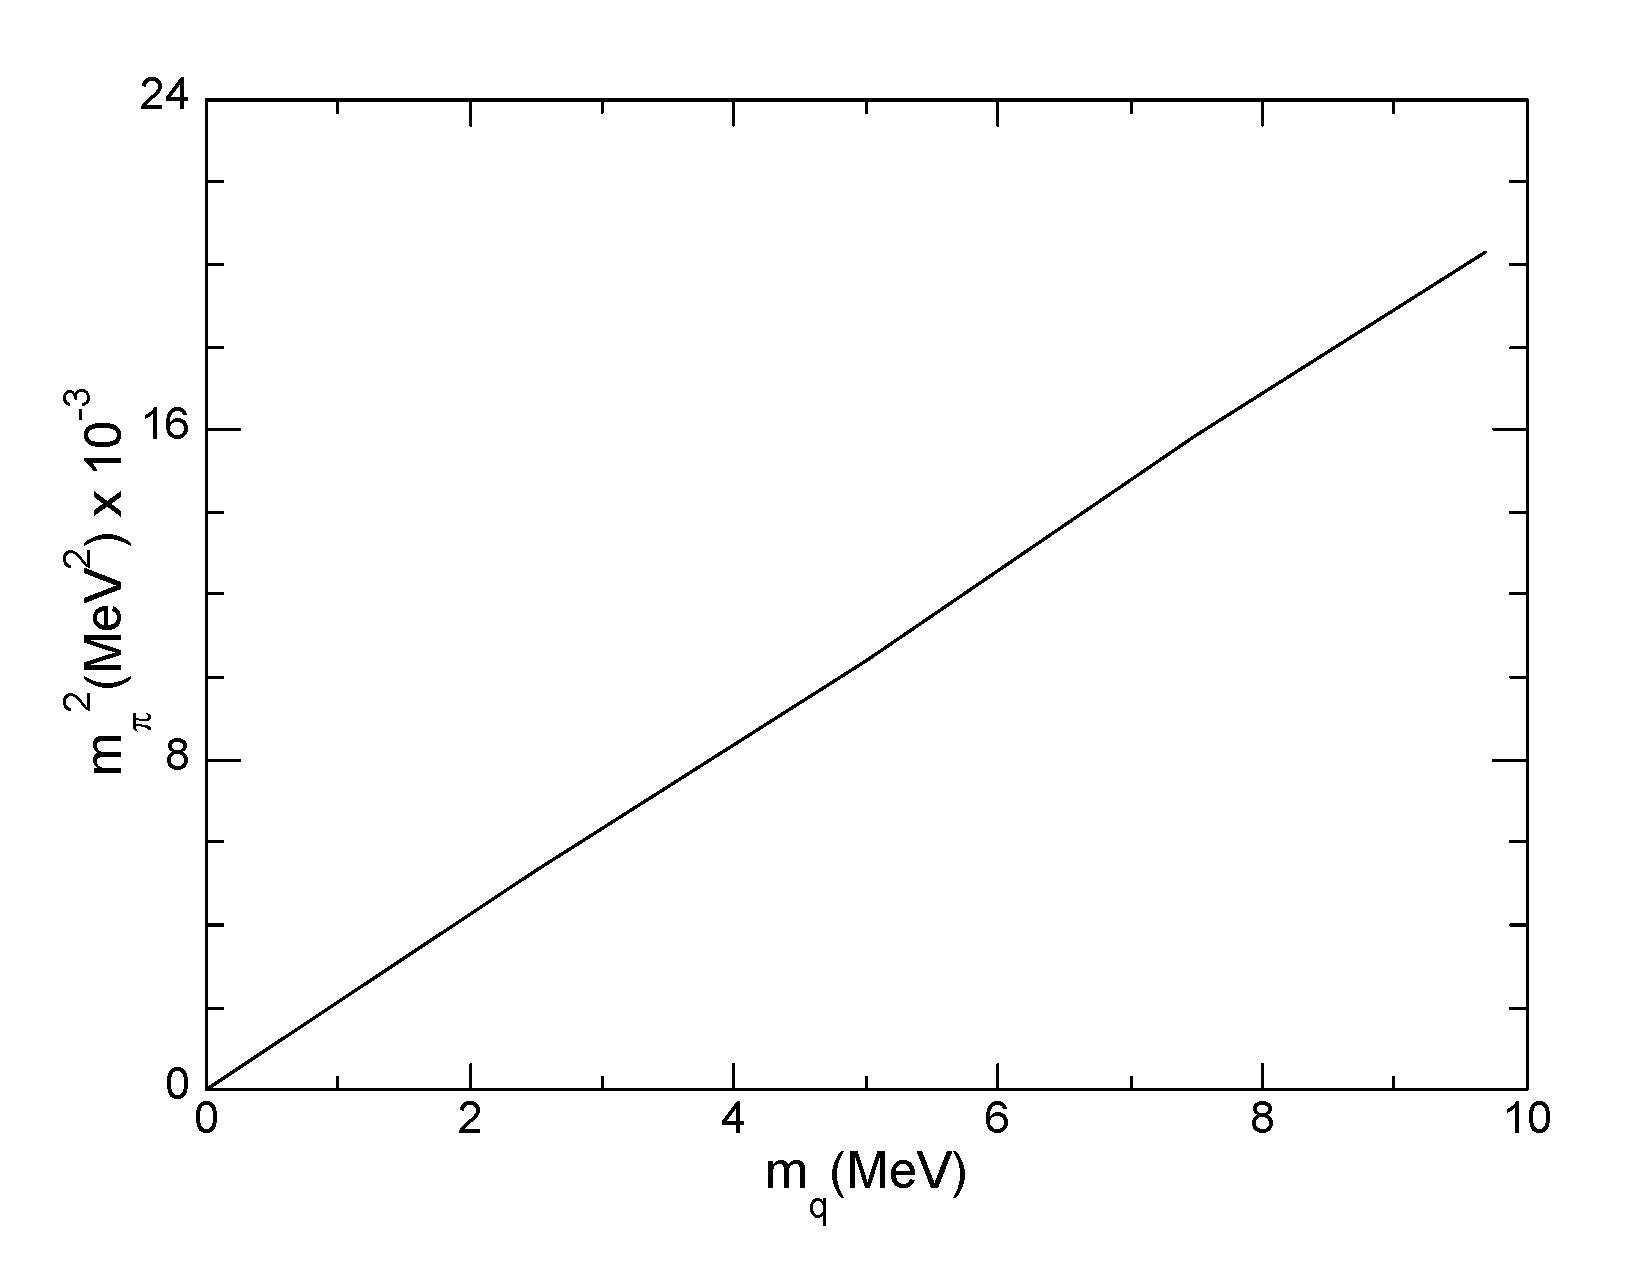
\includegraphics[width=300pt]{quarkvspion.pdf}}
\caption{Plot of $m_{\pi}^{2}$ vs $m_{q}$ yields a straight line from which the pion decay constant $f_{\pi}$ is calculated using (\ref{eq:GOR}).}
\label{fig:GOR}
\end{figure}

%\begin{figure}
%\center{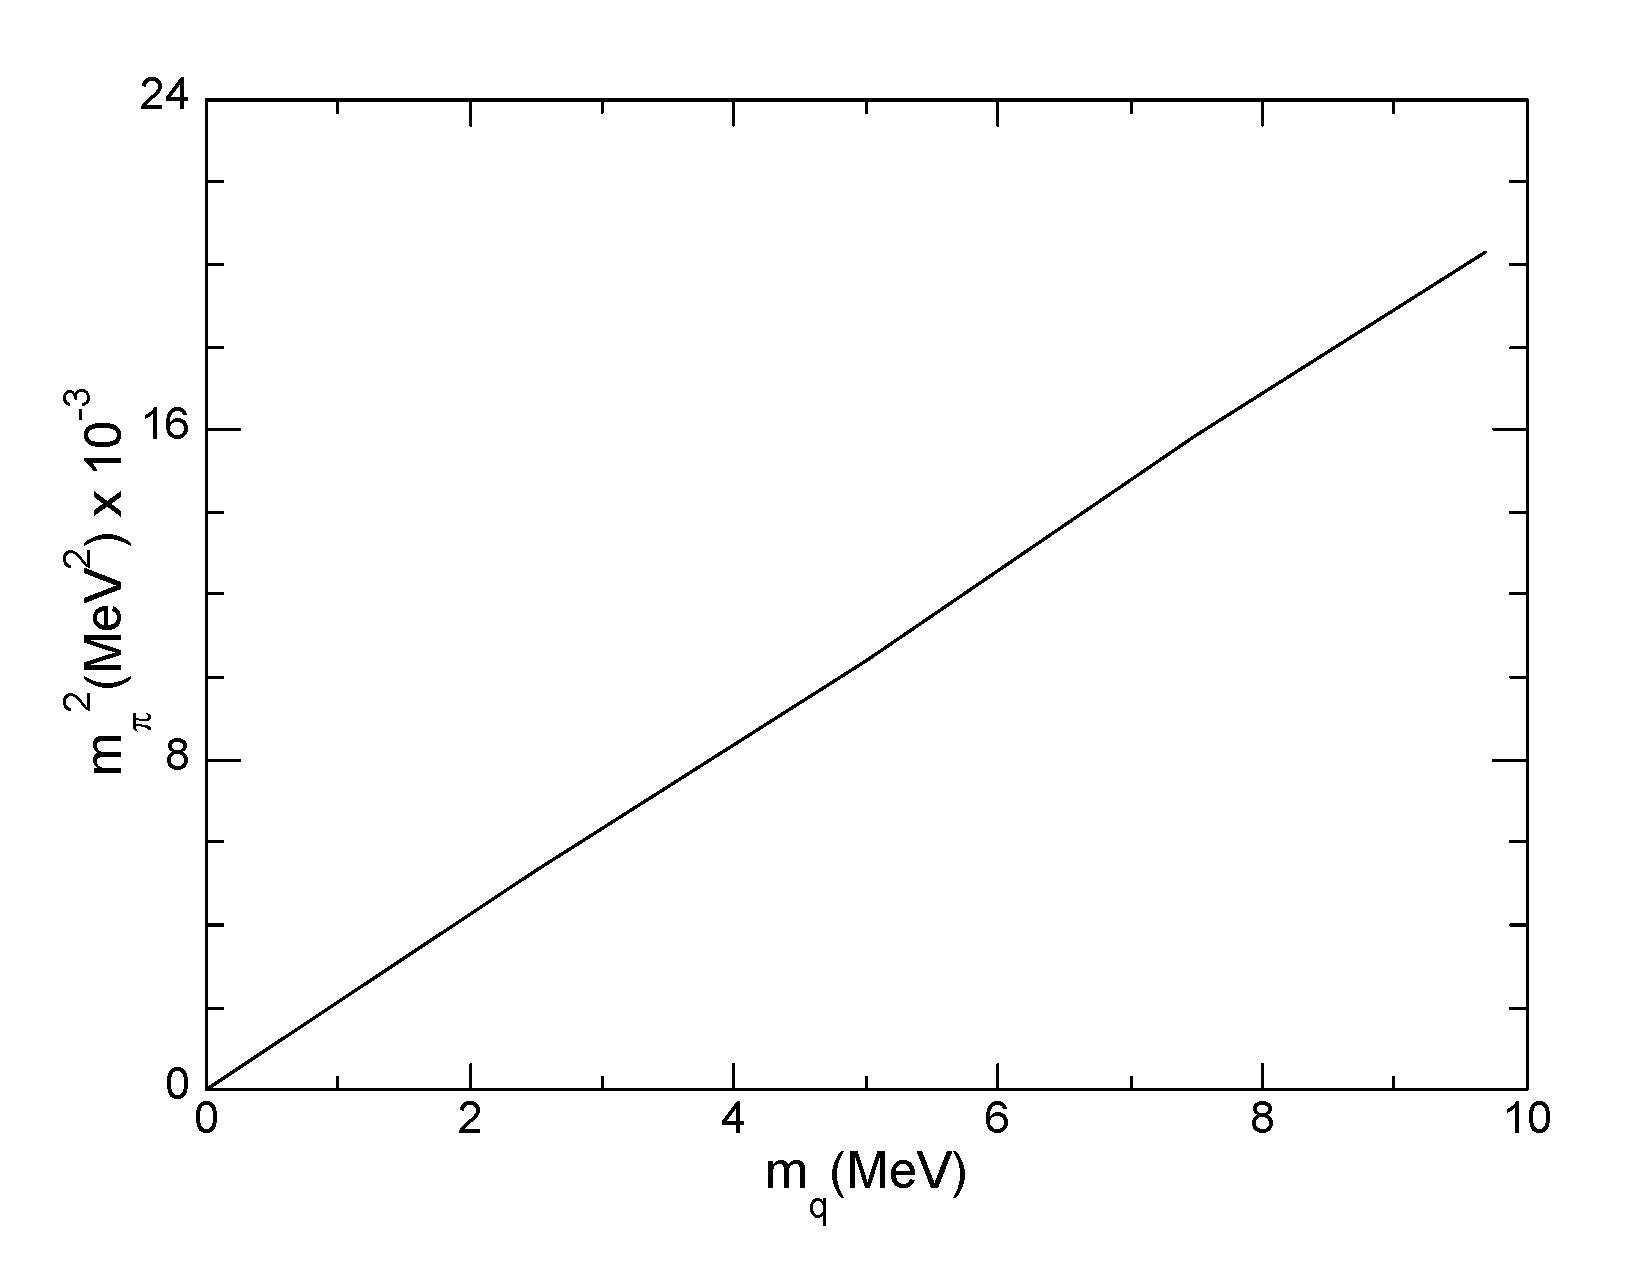
\includegraphics[width=300pt]{quarkvspion.pdf}}
%\caption{Plot of $m_{\pi}^{2}$ vs $m_{q}$ yields a straight line from which the pion decay constant $f_{\pi}$ is calculated using (\ref{eq:GOR}).}
%\label{fig:GOR}
%\end{figure}